\begin{frame}
	\note{
		\begin{itemize}
			\item go back to geometry class in high school
			\item right triangles, Pythagorean triples
			\item is there a nice way to generate Pythagorean triples?
		\end{itemize}
	}

	\begin{center}
		\begin{tikzpicture}[
				thought/.style = {
						cloud callout,
						fill = white,
						align = center,
						aspect = 2.5,
						inner sep=5pt,
						draw,
					}
			]
			\node[anchor=south west,inner sep=0] (image) at (0,0) {
				
\includegraphics[width=.8\textwidth]{images/caroline-adam-in-class.jpg}};

			\useasboundingbox (-1, -1) rectangle (9, 7.5);

			\node<2-> [fill = white, inner sep = 5pt] at (4, 0) {
				\rotatebox{-4}{\tikz[scale=.4]{
						\draw (0,0)
						to ["3"] (0, 3)
						to ["5"] (4,0)
						to ["4"] (0, 0);
					}}

				\onslide<3->{\rotatebox{10}{\tikz[scale=.3]{
							\draw (0,0)
							to ["5"] (0, 5)
							to ["13"] (12, 0)
							to ["12"] (0, 0);
						}}}
			};

			% caroline
			\node (caroline) at (2.3, 3.5);
			\node<4->[
				thought, callout absolute pointer=(caroline.north west)
			] at (1.7, 5.5) {I wonder if there \\ are more solutions?};

			% adam
			\node (adam) at (4.8, 4);
			\node<5->[
				thought, callout absolute pointer=(adam.north east)
			] at (6.5, 6) {When is recess?};
		\end{tikzpicture}
	\end{center}

	\note{You can trivially generate more solutions by multiplying all the sides by a constant.}

	\note{You want to do better.}

\end{frame}

\begin{frame}[t]
	\frametitle{Generating Primitive Pythagorean Triples}

	\textbf{Goal}: find all relatively prime $x, y, z \in \Z$ such that

	\begin{align*}
		z^2            & = x^2 + y^2                                                                            \\
		\onslide<2-8>{ & = \underbrace{(x + i y)}_\alpha \, \underbrace{(x - i y)}_\beta & \text{over $\Z[i]$}}
	\end{align*}

	\note{You're a very precocious 9th grader, so you obviously immediately recognize this as a factoring problem in the Gaussian integers.}

	\begin{overprint}

		\onslide<3-4>

		\begin{align*}
			\text{$x$ and $y$ relatively prime} \implies
			 & \text{$\alpha$ and $\beta$ relatively prime}            \\
			\onslide<4>{
				z^2 = \alpha \beta \implies
			 & \alpha = \gamma^2 \quad {\color{gray} \gamma \in \Z[i]}
			}
		\end{align*}

		\onslide<5->

		\begin{columns}
			\begin{column}{.5\textwidth}

				\begin{align*}
					\alpha        & = \gamma^2                                                                    \\
					\onslide<6->{ & = (a + bi)^2                                        \\}
					\onslide<7->{ & = \underbrace{(a^2 - b^2)}_x + \underbrace{2ab}_y i}
				\end{align*}
			\end{column}

			\begin{column}{.5\textwidth}
				\onslide<8->{
					\begin{align*}
						x & = a^2 - b^2 \\
						y & = 2 ab      \\
						z & = a^2 + b^2
					\end{align*}

				}
			\end{column}
		\end{columns}

		\onslide<9->

		\vskip-2em

		\begin{center}
			\def\arraystretch{1.3}
			\begin{tabular}{c|c|r}
				$a$ & $b$ &                      \\
				\hline
				$2$ & $1$ & $3^2 + 4^2 = 5^2$    \\
				$3$ & $2$ & $5^2 + 12^2 = 13^2$  \\
				% $3$ & $1$ & $8^2 + 6^2 = 10^2$   \\
				$4$ & $3$ & $7^2 + 24^2 = 25^2$  \\
				$4$ & $2$ & $12^2 + 16^2 = 20^2$ \\
				$4$ & $1$ & $15^2 + 8^2 = 17^2$
			\end{tabular}
		\end{center}

	\end{overprint}

	\note{
		\begin{itemize}
			\item You're feeling pretty good about yourself, Adam gets to go to recess, but I want to linger a bit on what happened here.
			\item Even if you didn't follow every step, the important part is that we started with a problem involving the integers, translated it into a problem about factoring in a larger ring, and got results about the integers.
			\item This is the essence of algebraic number theory
		\end{itemize}
	}
\end{frame}

\begin{frame}[t]
	\bigskip

	\tikz[
		quotes mean pin,
		annotation/.style = {
				font =\normalfont\normalsize,
				align = center,
			},
		highlight/.style = {fg = fg, fill = bg}
	]{
		\useasboundingbox (-4, 1) rectangle (7, -3);

		\usebeamerfont{frametitle}
		\usebeamercolor{frametitle}
		\node [alt=<2>{highlight}{}] (a) {Algebraic};
		\node [alt=<3>{highlight}{}, right = -.1em of a] (b) {Number Theory};

		\node<2-> [annotation, below left=3em and 1em of a.east] (aLabel) {Using tools from algebra like \\ rings and field extensions};

		\node<3-> [annotation, below right=2em and 2em of b.west] (bLabel) {Generating insight about \\ the integers and the primes};

		\draw<2-> (a.south) -- (aLabel.north);
		\draw<3-> (b.south) -- (bLabel.north);
	}

	\note{
		\begin{itemize}
			\item If that didn't make sense to you, that's fine
			\item The important part: we started with a problem involving the integers, translated it into a problem about factoring in a larger ring, and got results about the integers
			\item This is the essence of algebraic number theory
		\end{itemize}
	}

	\note{And this is a nice romantic vision of the field, but the book I was using to learn this material opens with a much more pragmatic definition:}

	\begin{center}
		\only<4->{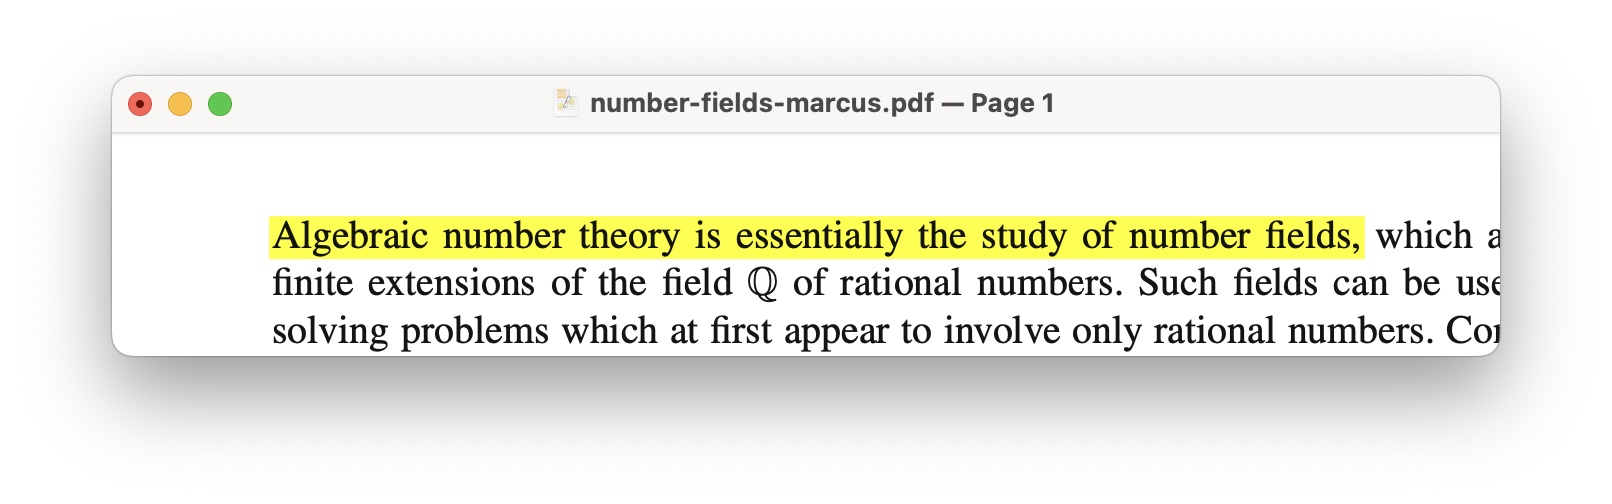
\includegraphics[width=\textwidth]{images/marcus-first-sentence.jpg}}
	\end{center}

\end{frame}

\begin{frame}
	\frametitle{Outline}

	\tableofcontents[pausesections]

	\note{
		\begin{enumerate}
			\item We'll start with a crash course in rings, because, unsuprisingly, you need some algebra to do algebraic number theory
			\item Then we'll talk a bit about number fields and number rings, which are the things that Marcus says algebraic number theory is all about.
			\item Next we'll talk about this thing called the ideal class group.
			\item This talk isn't intended to be comprehensive. My goal is really that I pique your interest and that you go read my paper when it comes out.
		\end{enumerate}
	}
\end{frame}
